\documentclass[aspectratio=169,11pt]{beamer}

% ============================================================
% Theme
% ============================================================
\usetheme{Madrid}
\usecolortheme{seahorse}
\setbeamertemplate{navigation symbols}{}



% Improve alert contrast on light themes
\setbeamercolor{block title alerted}{bg=red!15, fg=black}
\setbeamercolor{block body alerted}{bg=red!5, fg=black}
\setbeamercolor{alerted text}{fg=red!80!black}

% ============================================================
% Encoding (pdfLaTeX-safe)
% ============================================================
\usepackage[utf8]{inputenc}
\usepackage[T1]{fontenc}
\usepackage{lmodern}

% ============================================================
% Packages
% ============================================================
\usepackage{amsmath}
\usepackage{xcolor}
\usepackage{listings}
\usepackage{tikz}
\usetikzlibrary{positioning,arrows.meta}

% ============================================================
% Listings (Java)
% ============================================================
\lstset{
	language=Java,
	basicstyle=\ttfamily\small,
	frame=single,
	breaklines=true,
	columns=fullflexible,
	keywordstyle=\color{blue},
	commentstyle=\color{gray!70!black},
	stringstyle=\color{red!70!black},
	showstringspaces=false,
	backgroundcolor=\color{gray!5}
}

% ============================================================
% Small helper (pdfLaTeX-safe)
% ============================================================
\newcommand{\warn}{\Large\textbf{\alert{!}}}

% ============================================================
% Title
% ============================================================
\title{Concurrency \& Distributed Systems}
\subtitle{Week 2 --- Part 4: Race Conditions}
\author{Dr. Mohamad Aoude}
\institute{Lebanese University \\ Faculty of Engineering}
\date{\today}

% ============================================================
\begin{document}
	
	% ============================================================
	\begin{frame}
		\titlepage
	\end{frame}
	
	% ============================================================
	\begin{frame}
		\frametitle{Block 4 --- The Intentional Bug}
		\begin{center}
			\Large Today we intentionally break correctness.
		\end{center}
		\vspace{6mm}
		\begin{block}{Goal}
			Understand why correct coordination does NOT guarantee correct data.
		\end{block}
	\end{frame}
	
	% ============================================================
	\begin{frame}
		\frametitle{What Is a Race Condition?}
		\begin{block}{Definition}
			A race condition occurs when the outcome depends on uncontrolled thread timing.
		\end{block}
		\vspace{3mm}
		\textbf{Real-world example:} Two users booking the \emph{last seat} on a flight $\rightarrow$ both succeed $\rightarrow$ overbooking.
		\vspace{4mm}
		Requires:
		\begin{itemize}
			\item Shared mutable state
			\item At least one write
			\item No synchronization protecting it
		\end{itemize}
		\vspace{3mm}
		\begin{center}
			\Large Different interleavings $\Rightarrow$ different results.
		\end{center}
	\end{frame}
	
	% ============================================================
	\begin{frame}
		\frametitle{The Hidden Problem: \texttt{count++}}
		\begin{block}{Looks Simple}
			\texttt{count++}
		\end{block}
		\vspace{4mm}
		Actually expands to:
		\begin{enumerate}
			\item Read count
			\item Add 1
			\item Write result
		\end{enumerate}
		\vspace{2mm}
		{\footnotesize\alert{Note:} at the JVM level this becomes multiple operations (e.g., load / add / store) $\Rightarrow$ not atomic.}
		\vspace{4mm}
		\begin{center}
			\Large This is NOT atomic.
		\end{center}
	\end{frame}
	
	% ============================================================
	\begin{frame}
		\frametitle{Visualizing the Lost Update}
		\begin{center}
			\small Initial value: \texttt{count = 5}
		\end{center}
		\vspace{2mm}
		
		\begin{center}
			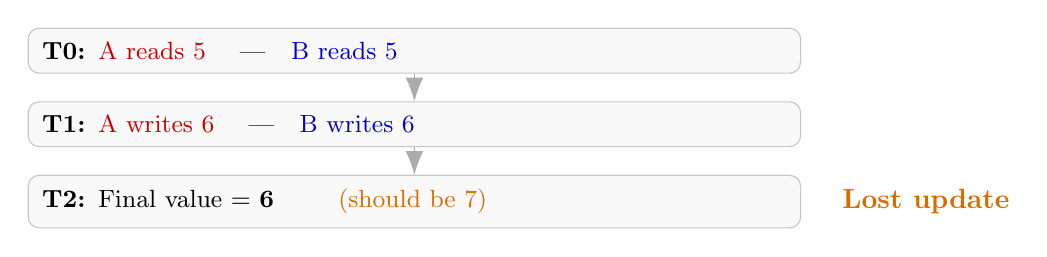
\begin{tikzpicture}[
				font=\small,
				box/.style={
					rounded corners,
					draw=gray!45,
					fill=gray!5,
					inner sep=5pt,
					text width=0.78\textwidth,
					align=left
				}
				]
				\node[box] (t0) {\textbf{T0:} \textcolor{red!80!black}{A reads 5} \quad|\quad \textcolor{blue!80!black}{B reads 5}};
				\node[box, below=3.5mm of t0] (t1) {\textbf{T1:} \textcolor{red!80!black}{A writes 6} \quad|\quad \textcolor{blue!80!black}{B writes 6}};
				\node[box, below=3.5mm of t1] (t2) {\textbf{T2:} Final value = \textbf{6} \hspace{6mm} \textcolor{orange!85!black}{(should be 7)}};
				
				\draw[-{Latex[length=3mm]}, gray!65] (t0) -- (t1);
				\draw[-{Latex[length=3mm]}, gray!65] (t1) -- (t2);
				
				\node[anchor=west, font=\bfseries, text=orange!85!black] at ([xshift=4mm]t2.east) {Lost update};
			\end{tikzpicture}
		\end{center}
		
		\vspace{2mm}
		\begin{block}{Key idea}
			Two correct-looking increments can produce one incorrect final result.
		\end{block}
	\end{frame}
	
	% ============================================================
	\begin{frame}
		\frametitle{Two Threads — One Variable}
		Initial value: \texttt{count = 5}
		\vspace{2mm}
		\begin{itemize}
			\item<+-> Thread A reads 5
			\item<+-> Thread B reads 5
			\item<+-> Thread A writes 6
			\item<+-> Thread B writes 6
		\end{itemize}
		\vspace{3mm}
		\begin{block}{Result}
			One increment is lost.
		\end{block}
	\end{frame}
	
	% ============================================================
	\begin{frame}
		\frametitle{Common Misconception}
		\begin{block}{Misconception}
			\textbf{“If I use \texttt{join()}, my result must be correct.”}
		\end{block}
		\vspace{3mm}
		\begin{block}{Reality}
			\texttt{join()} guarantees completion and visibility, \textbf{not} mutual exclusion or atomicity.
		\end{block}
	\end{frame}
	
	% ============================================================
	\begin{frame}[fragile]
		\frametitle{Intentional Race --- Coding Task}
		\begin{lstlisting}
			class Counter {
				static int count = 0;
			}
			Runnable task = () -> {
				for (int i = 0; i < 10000; i++) {
					Counter.count++;}
			};
			Thread[] threads = new Thread[10];
			for (int i = 0; i < 10; i++) {
				threads[i] = new Thread(task);
				threads[i].start();
			}
			for (int i = 0; i < 10; i++) {
				threads[i].join();
			}
			System.out.println("Expected: 100000");
			System.out.println("Actual:   " + Counter.count);\end{lstlisting}
	\end{frame}
	
	% ============================================================
	\begin{frame}
		\frametitle{Expected vs Actual}
		\begin{block}{Expected}
			100000
		\end{block}
		\begin{block}{Actual}
			Varies every run:
			\begin{itemize}
				\item 97342
				\item 98901
				\item 99512
			\end{itemize}
		\end{block}
		\vspace{3mm}
		\begin{alertblock}{\warn\ \textbf{Silent Corruption}}
			No crash. No exception. Just wrong.
		\end{alertblock}
	\end{frame}
	
	% ============================================================
	\begin{frame}
		\frametitle{Important Observation}
		\begin{itemize}
			\item All threads completed (\texttt{join()} used)
			\item Memory visibility guaranteed
			\item Yet result is incorrect
		\end{itemize}
		\vspace{5mm}
		\begin{block}{Critical Insight}
			Completion does NOT imply atomicity.
		\end{block}
	\end{frame}
	
	% ============================================================
	\begin{frame}
		\frametitle{Why \texttt{join()} Did Not Save Us}
		\texttt{join()} guarantees:
		\begin{itemize}
			\item Completion ordering
			\item Memory visibility (\emph{happens-before})
		\end{itemize}
		\vspace{4mm}
		\texttt{join()} does NOT guarantee:
		\begin{itemize}
			\item Mutual exclusion
			\item Atomic operations
		\end{itemize}
		\vspace{4mm}
		\begin{center}
			\Large Coordination $\neq$ Protection
		\end{center}
		\vspace{2mm}
		{\footnotesize Recall: \texttt{join()} enforces visibility, not safety.}
	\end{frame}
	
	% ============================================================
	\begin{frame}
		\frametitle{Debugging Prompt}
		Insert temporary print statements:
		\begin{itemize}
			\item Print thread name
			\item Print value before increment
		\end{itemize}
		\vspace{3mm}
		\textbf{What you will observe:} multiple threads read the same value, then overwrite each other.
		\vspace{4mm}
		\begin{block}{Overwrite Pattern (Example)}
			\renewcommand{\arraystretch}{1.2}
			\begin{tabular}{lcc}
				\textbf{Thread} & \textbf{Reads} & \textbf{Writes} \\
				\hline
				A & 5 & 6 \\
				B & 5 & 6 \\
			\end{tabular}
		\end{block}
		\vspace{2mm}
		\begin{block}{Reality}
			This is silent corruption.
		\end{block}
	\end{frame}
	
	% ============================================================
	\begin{frame}
		\frametitle{Formal Conditions for Race}
		A race condition exists when:
		\begin{enumerate}
			\item<+-> Two or more threads access the same variable
			\item<+-> At least one access is a write
			\item<+-> There is no synchronization
		\end{enumerate}
		\vspace{4mm}
		\begin{block}{Rule}
			If \textbf{any one condition is missing}, the race cannot occur.
		\end{block}
		\vspace{2mm}
		\begin{itemize}
			\item No shared state $\rightarrow$ thread-local variables
			\item No writes $\rightarrow$ read-only configuration
			\item With synchronization $\rightarrow$ \texttt{synchronized}, \texttt{AtomicInteger}, locks, etc.
		\end{itemize}
	\end{frame}
	
	% ============================================================
	\begin{frame}[fragile]
		\frametitle{Preview: Fixing It (Before / After)}
		\begin{columns}[T,onlytextwidth]
			\column{0.48\textwidth}
			\begin{block}{Before (Unsafe)}
\begin{lstlisting}
Counter.count++; // not atomic
\end{lstlisting}
			\end{block}
			
			\column{0.52\textwidth}
			\begin{block}{After (Safe)}
\begin{lstlisting}
// Option A: synchronized
synchronized(lock) {
		Counter.count++;
	}
// Option B: AtomicInteger
	AtomicInteger c = new AtomicInteger();
	c.incrementAndGet();
\end{lstlisting}
			\end{block}
		\end{columns}
		
		\vspace{1mm}
		\begin{center}
			\small Full solution next lecture.
		\end{center}
	\end{frame}
	
	% ============================================================
	\begin{frame}[fragile]
		\frametitle{Thread Dump Lab}
		Run:
		\begin{block}{Terminal}
			jps \\
			jstack -l <PID> > dump.txt
		\end{block}
		
		\vspace{1mm}
		\textbf{Example snippet:}
		\begin{lstlisting}[language={},basicstyle=\ttfamily\footnotesize]
			"Contender" #16  BLOCKED
			waiting to lock <0x000000076b>
		\end{lstlisting}
		
		\vspace{1mm}
		\begin{block}{Legend}
			\begin{itemize}
				\item \textbf{BLOCKED}: trying to enter a \texttt{synchronized} region but cannot
				\item \textbf{waiting to lock}: wants a monitor it does not own
				\item \textbf{\texttt{<0x...>}}: identifier for the monitor object
			\end{itemize}
		\end{block}
	\end{frame}
	
	% ============================================================
	\begin{frame}
		\frametitle{Guided Dump Analysis}
		\begin{itemize}
			\item Which thread is BLOCKED?
			\item On what object (monitor)?
			\item Who owns the monitor?
			\item How many RUNNABLE threads exist?
		\end{itemize}
		\vspace{5mm}
		Connect to:
		\begin{itemize}
			\item Lifecycle states
			\item Monitor ownership
		\end{itemize}
	\end{frame}
	
	% ============================================================
	\begin{frame}
		\frametitle{Micro Quiz}
		\begin{enumerate}
			\item Can a TERMINATED thread restart?
			\item Does \texttt{sleep()} release locks?
			\item Is RUNNABLE equal to executing?
			\item Does priority guarantee order?
			\item Is \texttt{count++} atomic?
		\end{enumerate}
	\end{frame}
	
	% ============================================================
	\begin{frame}
		\frametitle{Block 4 Summary}
		\begin{itemize}
			\item Race conditions cause silent corruption
			\item \texttt{join()} ensures completion, not safety
			\item \texttt{count++} is not atomic
			\item Shared mutable state requires synchronization
		\end{itemize}
		\vspace{5mm}
		\begin{block}{Key Insight}
			Concurrency errors are often invisible.
		\end{block}
	\end{frame}
	
	% ============================================================
	\begin{frame}
		\frametitle{One Rule to Remember}
		\begin{center}
			\Large
			If multiple threads write shared data,\\
			you MUST synchronize access.
		\end{center}
	\end{frame}
	
	
	\begin{frame}
		\frametitle{The Uncomfortable Truth}
		
		We now know:
		
		\begin{itemize}
			\item Threads can interleave unpredictably
			\item \texttt{count++} is not atomic
			\item \texttt{join()} ensures completion, not correctness
			\item Race conditions cause silent corruption
		\end{itemize}
		
		\vspace{6mm}
		
		\begin{block}{The Problem}
			If multiple threads write shared data, correctness is not guaranteed.
		\end{block}
		
	\end{frame}
	\begin{frame}
		\frametitle{The Key Question}
		
		\begin{center}
			\Large
			How do we guarantee that\\
			only one thread modifies shared data at a time?
		\end{center}
		
		\vspace{8mm}
		
		\begin{block}{What We Need}
			\begin{itemize}
				\item Mutual exclusion
				\item Controlled access
				\item Deterministic behavior
			\end{itemize}
		\end{block}
		
	\end{frame}
	\begin{frame}
		\frametitle{From Chaos to Control}
		
		We introduced:
		
		\begin{itemize}
			\item Race conditions
			\item Lost updates
			\item Interleaving problems
		\end{itemize}
		
		\vspace{6mm}
		
		Next step:
		
		\begin{center}
			\Large
			Synchronization \\
			Locks \\
			Critical Sections
		\end{center}
		
	\end{frame}
	\begin{frame}
		\frametitle{Week 3 Preview --- Synchronization \& Locks}
		
		In Week 3 we will:
		
		\begin{itemize}
			\item Eliminate race conditions
			\item Understand intrinsic locks
			\item Protect critical sections
			\item Create and detect deadlocks
			\item Inspect threads using tools
		\end{itemize}
		
		\vspace{6mm}
		
		\begin{block}{Goal}
			Move from unpredictable behavior to controlled concurrency.
		\end{block}
		
	\end{frame}
	\begin{frame}
		\frametitle{One Final Thought}
		
		\begin{center}
			\Large
			Concurrency is not dangerous. \\
			Uncontrolled concurrency is.
		\end{center}
		
		\vspace{8mm}
		
		\begin{center}
			Week 3 --- We take control.
		\end{center}
		
	\end{frame}
	
\end{document}
